\begin{figure}[h]
    \centering % Center everything
    \includegraphics{plot1.eps}  % This is an unscaled image
    %\includegraphics[width=.8\textwidth]{plot1.eps}
            % This is scaled image, which will have width of 80 percent
            % of the textwidth.
            % The width can also be specified as 5cm,4in,3mm, etc.
    \caption{
        Example of a figure.
        %
        Note that for best results one should not have to do any scaling
            for the figures, which appear in the documents, as the lines
            and fonts are not rendered as they were intended to.
    }
    \label{fig:plot1} % This label is later used for cross-referencing
\end{figure}
